% Needs graphicx. Select the figures appropriate for the paper.
\begin{figure*}[!htbp]
\centering
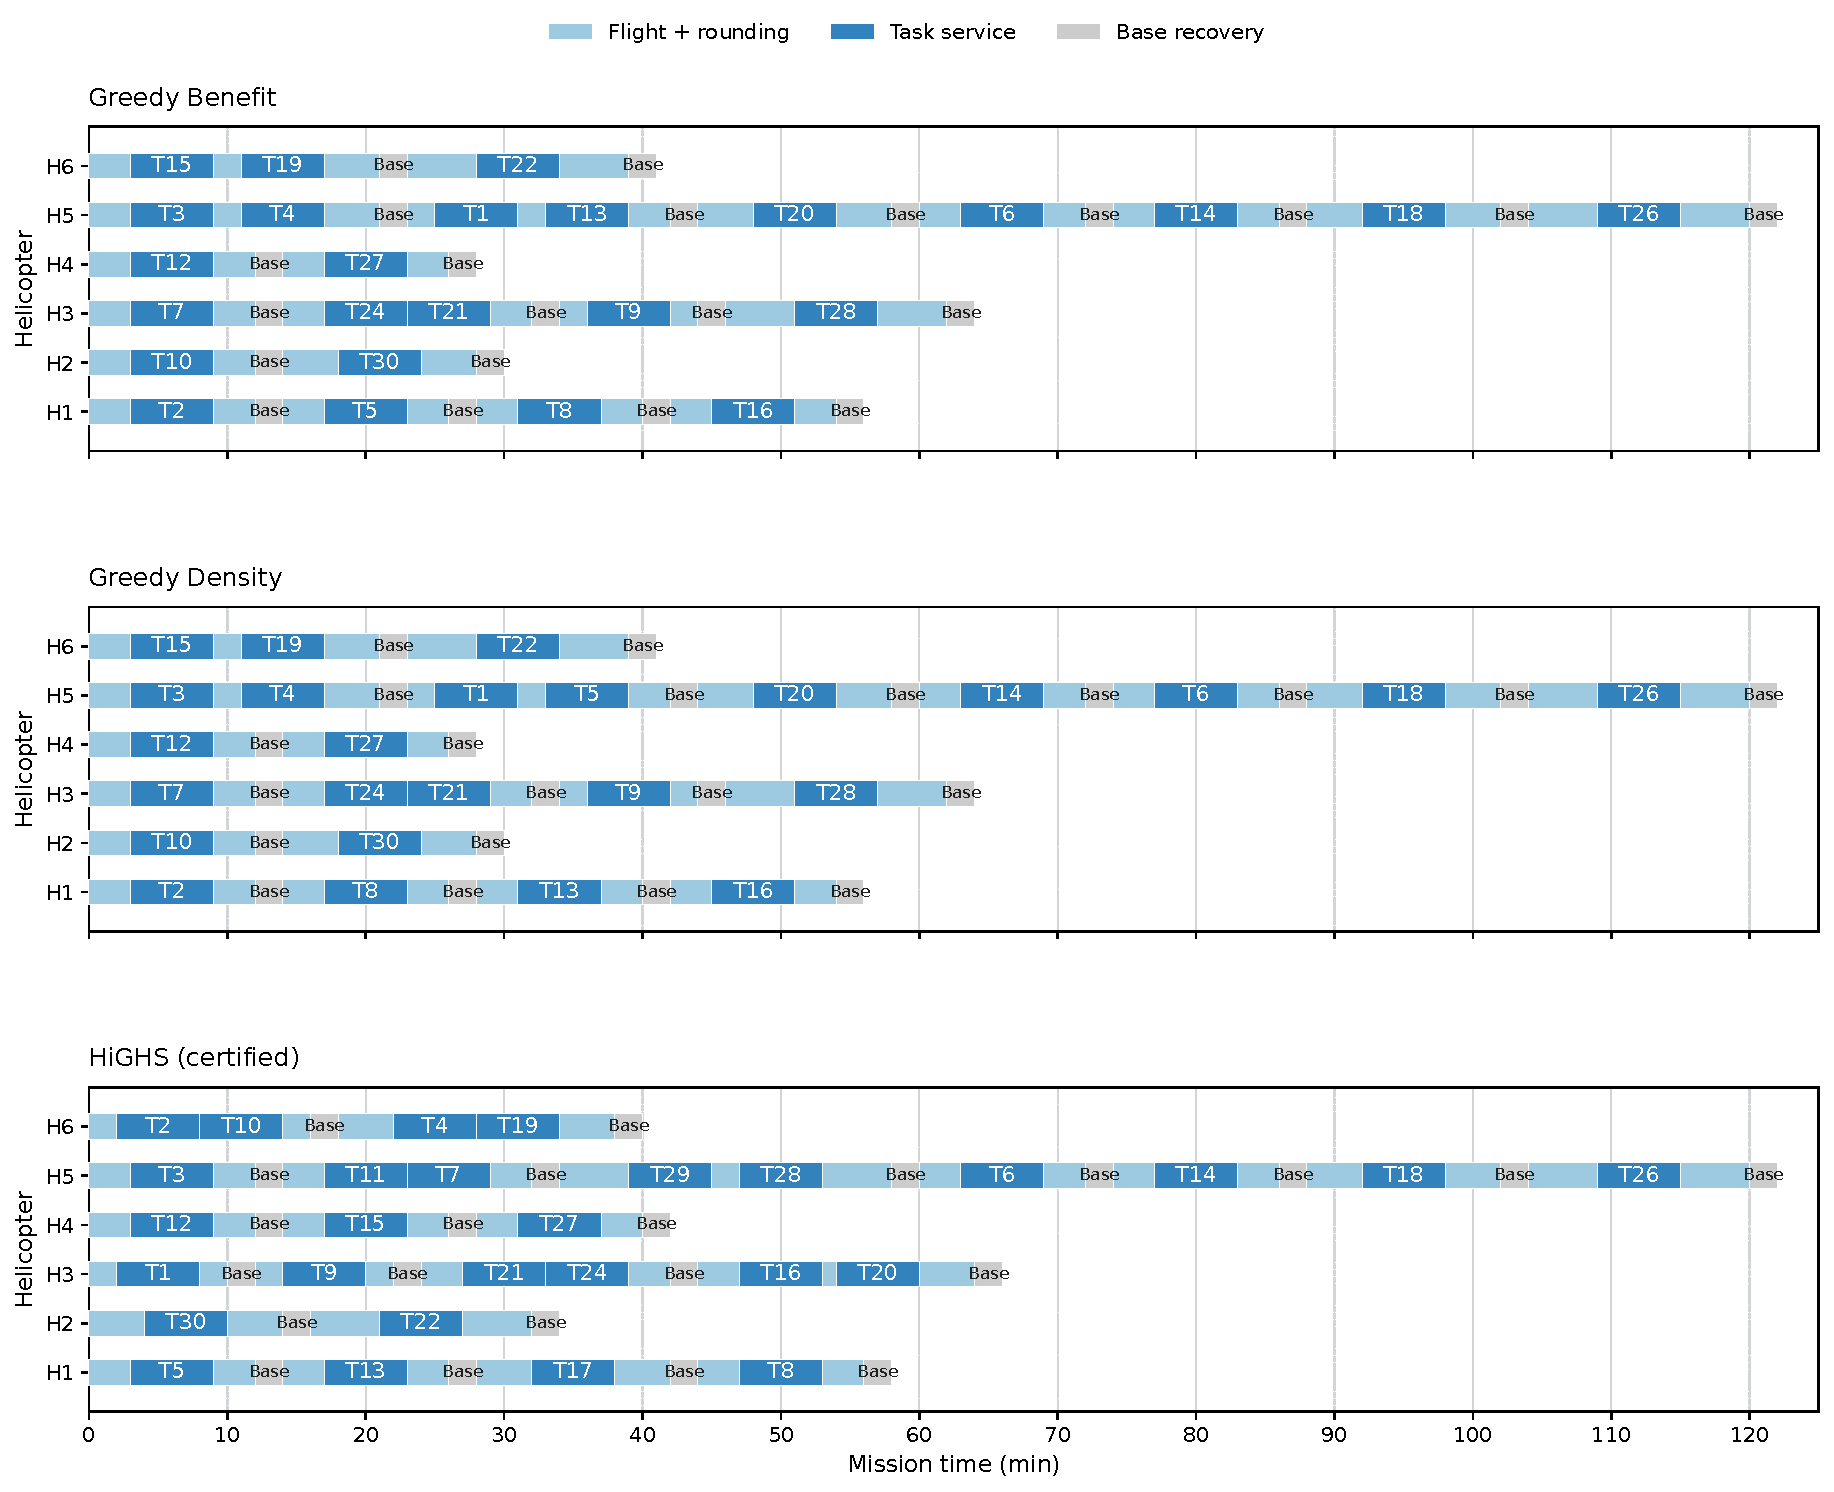
\includegraphics[width=\textwidth]{GPS_gantt_comparison_three_methods.pdf}
\caption{Schedules for the fixed GPS scenario under Greedy Benefit, Greedy Density
and HiGHS. All panels use the same mission-time interval and fleet identifiers.
Recorded activity starts and completion times, and service and recovery durations,
are preserved. For display, the flight segment includes the time-grid rounding remainder. Reported flight metrics retain the original physical flight durations.}
\label{fig:gps-gantt-three-methods}
\end{figure*}

\begin{figure}[!htbp]
\centering
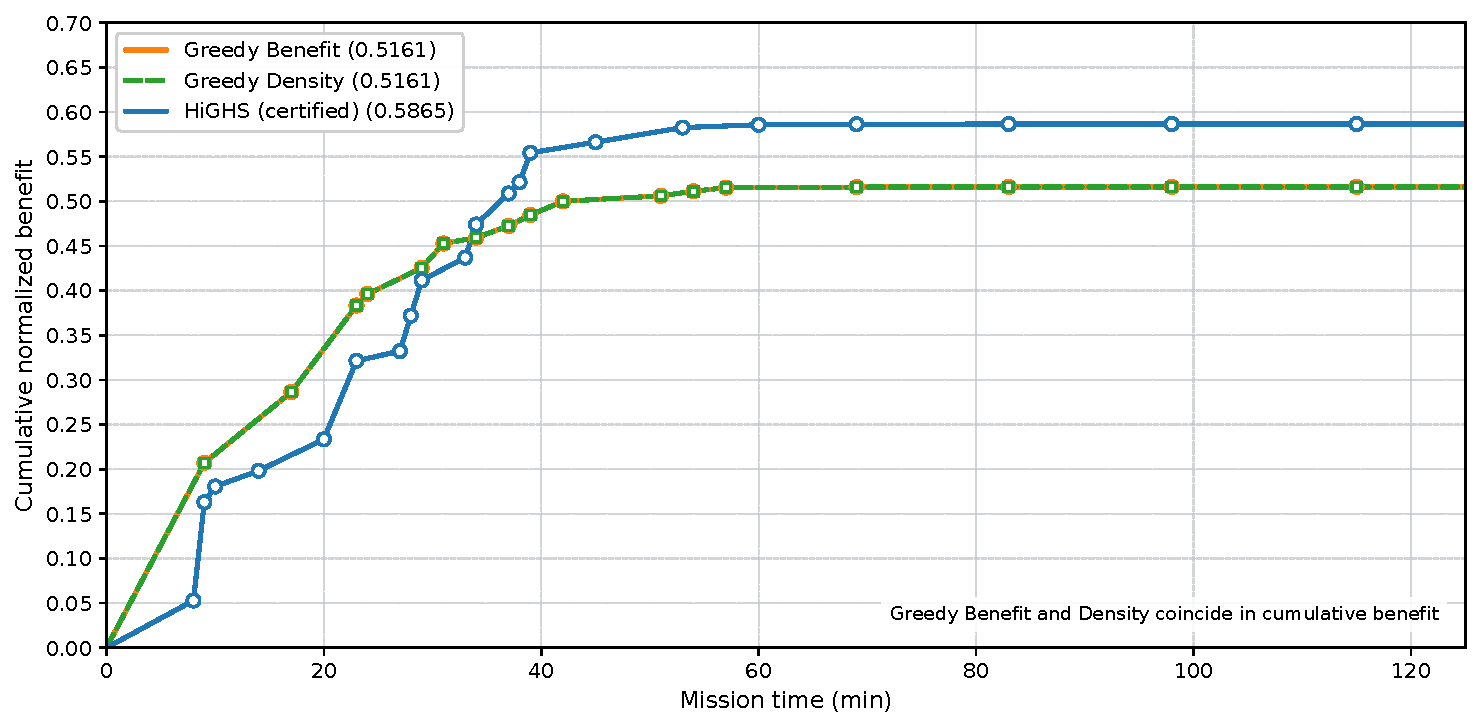
\includegraphics[width=\columnwidth]{GPS_cumulative_comparison_three_methods.pdf}
\caption{Cumulative normalized benefit in the fixed GPS scenario. Points show cumulative values at task completions; connecting lines are visual guides.
The two greedy histories can coincide even when their flight routes differ.
This is one fixed instance; no repeated-instance uncertainty bands are shown.}
\label{fig:gps-cumulative-three-methods}
\end{figure}

% Optional descriptive metrics; they do not share a common objective scale.
\begin{figure*}[!htbp]
\centering
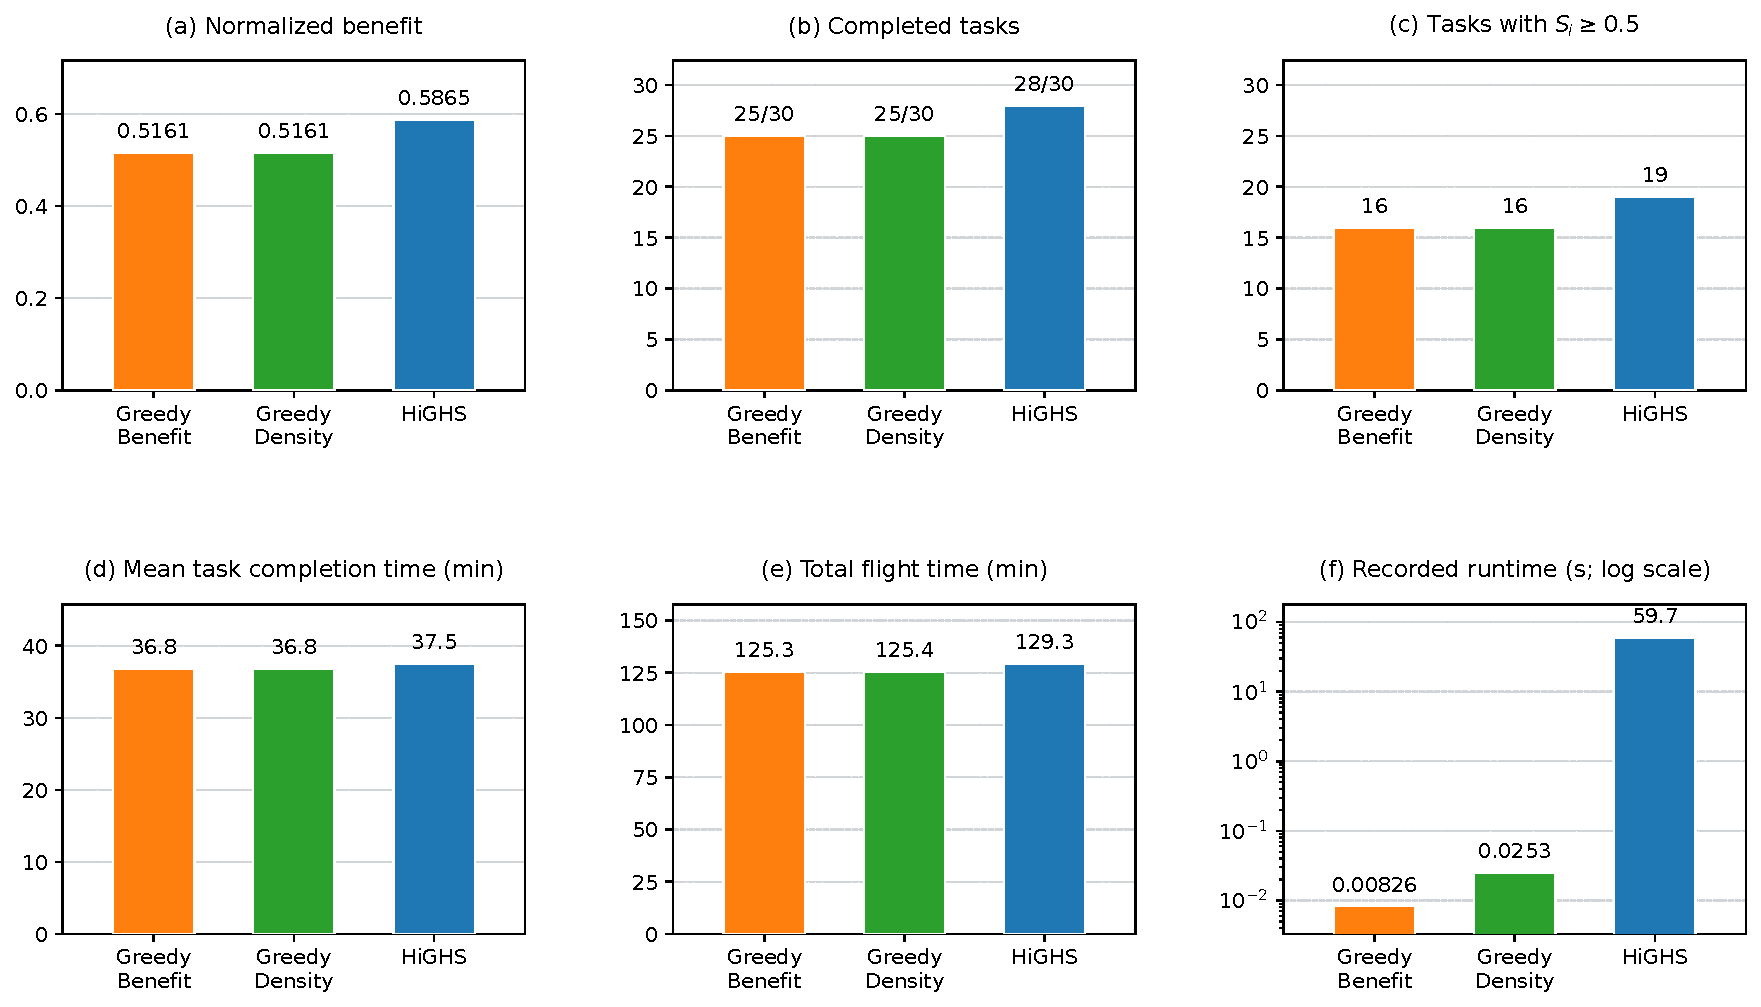
\includegraphics[width=\textwidth]{GPS_metrics_final.pdf}
\caption{Descriptive outcomes of the fixed GPS scenario. Task counts, completion
times, flight totals and recorded runtimes summarize the existing schedules.
HiGHS maximizes temporal benefit; the remaining metrics are not independent
optimization objectives. Runtime uses a logarithmic scale. No repeated-instance
error bars are inferred from this single scenario.}
\label{fig:gps-metrics}
\end{figure*}
